%        File: pnas1.tex
%     Created: Wed Apr 30 04:00 pm 2014 E
% Last Change: Wed Apr 30 04:00 pm 2014 E
%
\documentclass[letterpaper]{article} 
\usepackage{aaai} 
\usepackage{times} 
\usepackage{helvet} 
\usepackage{courier} 
\setlength{\pdfpagewidth}{8.5in} 
\setlength{\pdfpageheight}{11in} 
%%%%%%%%%%
% PDFINFO for PDFLATEX
% Uncomment and complete the following for metadata (your paper must compile with PDFLATEX)
\pdfinfo{
	/Title Inter-Task Effects Induce Bias in Crowdsourcing
	/Author Edward Newell
	/Keywords priming, framing, crowdsourcing
}


\usepackage{graphicx}
\usepackage{amsmath}
\usepackage{amssymb}
\usepackage{mathrsfs}
\usepackage{gensymb}
\usepackage{algorithm2e}
\usepackage{amsthm}
\usepackage{caption}

\newtheorem*{mydef}{Definition}

\usepackage{framed, color}
\usepackage{soul}
\usepackage[colorlinks=false, urlcolor=blue]{hyperref}
\usepackage{dcolumn}
\usepackage{multirow}
\usepackage{booktabs}
\newcolumntype{d}{D{.}{.}{4.0}}
\newcolumntype{s}{D{.}{.}{1.4}}

%\setlength{\parindent}{0cm}
%\setlength{\parskip}{4mm plus1mm minus1mm}

%%%%%%%%%%
% Section Numbers
% Uncomment if you want to use section numbers % and change the 0 to a 1 or 2
% \setcounter{secnumdepth}{0} %%%%%%%%%%
\title{Inter-Task Effects Induce Bias in Crowdsourcing}
\author{Edward Newell\footnote{bla} \and Derek Ruths\\
School of Computer Science, McGill University, Montreal, Canada\\
$^*$\texttt{edward.newell@mail.mcgill.ca}\\
}
%%%%%%%%%%
% Body of Paper Begins
\begin{document}

\maketitle
\section*{Abstract}
Microtask platforms allow researchers to engage participants quickly and 
inexpensively.
Workers on such platforms probably perform many tasks in succession,
so we investigate interactions between earlier tasks and later ones, which we 
call \textit{inter-task} effects.  
Existing research investigates many task design factors, such as 
\textit{framing}, on the quality of responses, but to our knowledge, does not 
address inter-task effects.  
We used a canonical image-labeling task on Amazon Mechanical Turk 
to measure the impact of inter-task and framing effects on the focus and 
specificity of labels that workers provide.
We found that inter-task effects had a much stronger impact than framing, 
and that workers provided more specific labels when labeling 
a series of images that were similar to one another.

\paragraph{Keywords:} priming, framing, crowdsourcing.
\section*{Introduction}
Microtask crowdsourcing platforms like Amazon Mechanical Turk (MTurk) make it 
possible to submit batches of small tasks to a large pool of human workers, 
who do the tasks for fun, a sense of purpose, and remuneration 
\cite{kazai2013analysis,Antin20122925}.  
Originally used to distribute clerical work, these platforms 
increasingly serve as a fast and cheap means to engage experimental 
participants in a research 
setting \cite{snow2008cheap}.  

The task requester can interact with the platform like a compute server, 
seamlessly 
integrating human and machine computation.  Researchers have put forward the 
term HPU (Human co-Processing Unit), viewing the introduction of 
microtask platforms as a new computing architecture
\cite{5543192}.  

Here, we highlight an important way in which HPUs differ from CPUs, with 
serious implications for the design of tasks.  It is well-known that people 
are subject to priming effects 
\cite{BJOP1796,No2007,beller1971priming} and, in particular, task-repetition effects
\cite{Gass1999549,sohn2001task}.  
We investigate the effect that previously completed tasks have on workers'
responses during subsequent ones. We call such effects 
\textit{inter-task effects}.  Inter-task effects would amount to a kind of
\textit{hysteresis}, meaning that HPU output is not only a function of the 
current input, but also of the history of inputs.

There has been considerable investigation into the factors that affect the 
quality and quantity of micro-task completion.  These include the level of 
pay \cite{kazai2013analysis}, training \cite{le2010ensuring}, screening of 
workers \cite{paolacci2010running}, and user-interface design 
\cite{Finnerty2013}.  Researchers have also investigated \textit{framing}, 
by testing the effects of disclosing the workflow context 
\cite{Kinnaird2012281}, and the purpose of tasks 
\cite{chandler2013breaking}.  To our knowledge, no study has investigated 
inter-task effects.

We investigated inter-task effects on the MTurk platform, using image-labeling 
tasks, one of the most common kinds of tasks on MTurk
\cite{chandler2013breaking,Berinsky2012351,Finnerty2013,paolacci2010running}.  
Workers were required to label images featuring 
food and culture.  We regard these tasks as consisting of an 
\textit{initial} and a \textit{test set}, but, crucially, no
distinction was made between these sets from the view of the worker.
We varied the images in the initial tasks, while keeping those in the test set 
the same, to analyze the effects that the initial tasks had on the 
content and specificity of labels attributed in the test set.

As a point of comparison, we subjected some groups of workers to a kind of
\textit{framing}, by disclosing a fictitious, semantically-loaded name for 
the requester funding the tasks.
The names were chosen to suggest the requester's interest in a specific 
aspect of the image content.  We expected this would cause workers 
to provide more labels, and greater specificity, relating to this 
``preferred'' content.

Surprisingly, we found that inter-task effects were much stronger than
framing.  Our results show that initial tasks can significantly alter the 
focus of worker's labels.  Interestingly, we find that inter-task
effects can be used to induce greater specificity.  Our results suggest that
workers attribute more specific labels when labeling a series of images that
that are more similar to one another.  This suggests that careful 
consideration should be given to the bundling of tasks when designing a study 
using a microtask platform.


\subsection*{Experimental Setup}
\begin{table}[t]
\centering
	\begin{tabular}{ l  l  l }
		\hline                       
		Treatment & Funder & Initial Image Set	\\ 
		\hline                       
		$\textsc{ambg}$ & None & Ambiguous\\
		$\textsc{cult}_{img}$ & None & Cultural\\
		$\textsc{cult}_{fund}$ & Cultural & Cultural\\
		$\textsc{cult}_{fund,img}$ & Cultural & Cultural\\
		$\textsc{ingr}_{img}$ & None & Ingredients\\
		$\textsc{ingr}_{fund}$ & Nutritional & Ingredients\\
		$\textsc{ingr}_{fund, img}$ & Nutritional & Ingredients\\
		\hline  
	\end{tabular}

	\caption{ \footnotesize{ 
		Workers were assigned uniformly at random to one of the 
		treatments listed above. 
		The full funder names used were 
		``The Global Foundation for Cultural Recognition'' and 
		``The National Foundation for Nutritional Awareness''.  
		The ambiguous, cultural, and ingredients initial image sets are shown 
		in \textbf{Figs. S2}, \textbf{S3}, and \textbf{S4}.
	}}
	\label{table:1}
\end{table}
We solicited 900 MTurk workers to perform image-labeling tasks relating to
food and culture.  The workers were randomly assigned to one of the treatments
shown in \textbf{Table 1}.  The treatments $\textsc{ingr}_{fund,img}$ and 
$\textsc{cult}_{fund,img}$ used (respectively) the image sets of 
$\textsc{ingr}_{img}$ and $\textsc{cult}_{img}$, but also 
incorporated framing.  The addition of framing did not have a substantial
impact on the results for these treatments, so we do not discuss 
$\textsc{ingr}_{fund,img}$ and $\textsc{cult}_{fund,img}$ further.

Workers from all treatments were shown brief instructions.  Depending on 
their treatment, workers were then 
shown the name of a research funder, or this step was skipped.
Next, workers were given a series of ten image-labeling tasks.  Each task 
required workers to privide five discriptive labels for an image.  For the 
purpose of analysis, we divided the tasks
into \textit{initial} and \textit{test} sets, comprising respectively the 
first five and last five tasks.  From the perspective of the worker, there 
was no distinction or interruption between the initial and test sets. 
Depending on the treatment, one of three sets of images was used for the
initial tasks, but the images in the test set were always the same.

The images from the test set contained prepared meals and featured a 
prominent, identifiable culture (see \textbf{Fig. S1}).
To identify the initial image sets, we use the names ``ambiguous'', 
``cultural'', and ``ingredients''.  The ambiguous set was chosen to
be similar to the test set, in the sense that it consisted of
images of prepared meals (see \textbf{Fig. S2}),  but its cultural 
features were less prominent.  The cultural set featured 
iconic cultural scenes, but no food at all (see \textbf{Fig. S3}).  Images from 
the ingredients set depicted separated ingredients, but, 
like the ambiguous set, avoided prominent cultural features (see 
\textbf{Fig. S4}).
\subsection*{Results}
\begin{figure*}
	\centering{
		\includegraphics[scale=0.70]{figs/orientation_specificity.pdf}
	\caption{\footnotesize{
		\textbf{A}) Percent label composition (culture- vs food-oriented 
		labels) for 
		various treatments.  
		\textbf{B}) Relative specificities of treatments,
		indicated along the abscissa, compared to those indicated above the 
		plot, according to \textbf{Eq. 2}.  The size of the bar indicates how 
		much more specific
		the labels from one treatment are compared to the other, and points 
		toward the more specific treatment.  Error bars
		indicate 95\% confidence intervals.
	}}
}
\end{figure*}


\paragraph{Earlier tasks oriented workers' focus during later tasks.} 
Since the initial images were chosen to emphasize either food (ingredients set)
or culture (cultural set), we looked for effects on the number of culture- and 
food-oriented labels that workers attributed to the test image set.

To this end, we constructed an ontology from the labels attributed to the 
test images.  In the ontology, edges point from more general labels to more 
specific ones.  For example, the ontology contains the path \texttt{food} 
$\to$ \texttt{ingredients} $\to$ \texttt{vegetables} $\to$ \texttt{tomato}.

Since food is a central feature 
of culture, our ontology contains many labels that have both \texttt{food}
and \texttt{culture} in their ancestry.  Nevertheless, there were many 
food-oriented labels, such as \texttt{bread}, which lacked specific cultural 
connections, as well as non-food, culture-oriented labels, such as 
\texttt{russian dolls}. 


When we tallied labels attributed to the first image of the test set, 
we found that workers from $\textsc{cult}_{img}$ produced significantly 
more culture-oriented labels and less food-oriented ones than those from
\textsc{ambg} (see \textbf{Fig. 1A}).  The inter-task effects were so 
strong that the proportion of food- and culture-oriented labels in 
$\textsc{cult}_{img}$ was essentially the reverse of that in \textsc{ambg},  
showing that inter-task effects \textit{can} profoundly alter workers' focus. 

\paragraph{Inter-task effects were stronger than framing effects.}
On the other hand, the labels attributed by 
$\textsc{ingr}_{fund}$ were not significantly different in composition from 
those attributed by $\textsc{cult}_{fund}$.  Workers from the
these treatments were told that the tasks were funded by, respectively, 
the ``Foundation for Nutritional Awareness'' and the ``Foundation for Cultural 
Recognition''.  We find it remarkable that inter-task effects were stronger
than those brought about by framing the tasks with reference to specific 
image content.

\paragraph{Earlier tasks influenced workers' level of specificity.} 
The ontology described in the previous section allows us to define the relative
specificity of two labels $\ell_1$ and $\ell_2$. We say that $\ell_2$ is more 
specific than $\ell_1$ if there is a \textit{directed path} from $\ell_1$ to 
$\ell_2$.  If there is no directed path between labels, we say they are  
\textit{non-comparable}.  For example, \texttt{tomato} was more specific than 
\texttt{food}, while \texttt{statue} and \texttt{food} were non-comparable.

We can then define the relative specificity of two workers with respect to 
test-image $i$ as $s_i(u,v)$:

\begin{align}
	s_i(u,v) = \sum_{\ell \in u(i) } \;
	\sum_{m \in v(i)} 
	\left(\mathbf{1}_{[\ell > m]} - \mathbf{1}_{[m>\ell]}\right),
	\label{eq:worker-specificity}
\end{align}
where $u(i)$ denotes the set of labels attributed by worker $u$ to image $i$, 
and $\mathbf{1}_{[\ell > m]}$ evaluates to 1 if $\ell$ is more specific than 
$m$, and 0 otherwise.
We can then define the relative specificity of two treatments, $\mathcal{U}$ 
and $\mathcal{V}$, with respect to the $i$th image, denoted $S_i(\mathcal{U},\mathcal{V})$, 
to be the mean relative specificity of two uniformly drawn workers:  
\begin{align}
	\hat{S}_i(\mathcal{U},\mathcal{V}) = 
	\frac{1}{|\mathcal{U}| |\mathcal{V}|}
	\sum_{u \in \mathcal{U}} \;
	\sum_{v \in \mathcal{V}} \;
		s_i(u,v).
		\label{eq:specificity}
\end{align}

The relative specificities of various treatments, based on \textbf{Eq. 2},
are shown in \textbf{Fig. 1B}.  We found that workers 
from \textsc{ambg} were more specific than workers from
either $\textsc{cult}_{img}$ or $\textsc{ingr}_{img}$.  Comparing
$\textsc{cult}_{img}$ to $\textsc{ingr}_{img}$, we found that workers from
$\textsc{ingr}_{img}$ were more specific.  This shows that inter-task 
effects do substantially influence the specificity of labels that workers 
provide.  We will return to this point below, where we propose a mechanism to 
explain these differences in specificity. 

\paragraph{Inter-task effects ``washed out'' quickly.}  
It would stand to reason that, as workers proceed through the test images, 
priming from the initial images would be ``washed out'', diminishing the 
observed inter-task effects.

\begin{figure}
	\centering{
	\includegraphics[scale=0.7]{figs/longitudinal_theta_excess-culture_cut_for_hcomp.pdf}
	\caption{\footnotesize{
		Excess cultural orientation ($\Delta_\mathbf{cult}$) of labels 
		attributed by $\textsc{cult}_{img}$ relative to those attributed by 
		\textsc{ambg} 
		($\Delta_\mathbf{cult}$ is defined in \textbf{Eq. 3}).  Error bars 
		indicate 95\% confidence intervals.
	}}
}
\end{figure}
To investigate the evolution of inter-task effects, we define the 
\textit{excess cultural orientation} to be the number of 
culture-oriented labels minus the number of food oriented ones.  This measures
how culture-oriented a given image is.  Of course, we must account for the 
fact that some images inherently carry more 
cultural content than others. In keeping with our notion of priming 
\textit{difference}, we calculate the excess cultural content for 
both $\textsc{cult}_{img}$ and \textsc{ambg}, and take their difference to be
the \textit{relative} excess cultural content, $\Delta_{cult}$.  Formally,
\begin{align}
	\begin{split}
	\Delta_{cult}(i) = \frac{1}{N}\left[ \sum_{w\in\textsc{cult}_{img}} \left(N_{w,cult}^{(i)} - N_{w,food}^{(i)}\right)\right. \\
\left.	- \sum_{w\in\textsc{ambg}} \left(N_{w,cult}^{(i)} - N_{w,food}^{(i)}\right)\right],
	\end{split}
\end{align}
where $N_{w,cult}^{(i)}$ stands for the number of culture-oriented labels 
attributed by worker $w$ to image $i$, while $N_{w,food}^{(i)}$ similarly 
counts food-oriented labels, and $N$ is the total number of labels in a 
treatment.  

We found $\Delta_{cult}$ was largest for the first test image, but dropped off 
rapidly, remaining positive but not to a statistically significant extent
(see \textbf{Fig. 2}).  

\paragraph{Inter-task similarity encouraged more specific labels.}
To continue with the analysis, we sought a measure of image similarity.  The 
characterization of image content is a deeply complex issue that has been 
approached by many disciplines 
\cite{panofsky1939studies,shatford1986analyzing,Tversky1977327,Jaimes20002}.
However, in the present study we are more interested how similar two 
sets of images are, \textit{with respect to the labeling task}, which is
simpler to operationalize than general perceptual similarity.  For this purpose
we measured the similarity between two sets of images by looking at the 
fraction of labels that they shared. 
Formally, to measure the similarity between two \textit{sets of images}, $X$ 
and $Y$, we computed the Jaccard index between the sets of labels attributed 
to them:
\begin{align}
	\text{Sim}(X,Y) = \frac{L(X) \cap L(Y)}{L(X) \cup L(Y)},
\end{align}
where $L(X)$ denotes the set of labels attributed to $X$.

\begin{table}
\centering
\begin{tabular}{ l  s s s s}

\toprule    
Image set   
& \multicolumn{1}{c}{Ambig.} 
& \multicolumn{1}{c}{Cultural} 
& \multicolumn{1}{c}{Ingr.}
& \multicolumn{1}{c}{Test} \\
  
\midrule

Ambiguous  & 1 & 0.0418 & 0.142 & 0.167 \\

Cultural  & 0.0418  & 1 & 0.0347 & 0.0561 \\

Ingredients  & 0.142  & 0.0347 & 1 & 0.110 \\

Test & 0.167  & 0.0561 & 0.110 & 1
\\
\bottomrule

\end{tabular}
\caption{\footnotesize{
Pairwise similarities of each image set based on the labels attributed to them (see \textbf{Eq. 4}).
}}
\label{table:2}
\end{table}

The pairwise similarities of the image sets are presented in \textbf{Table 2}. 
In particular, we draw the reader's attention to the similarity between the 
three initial sets and the test set.  The ambiguous set was the most similar 
to the test set, followed by the
ingredients set, while the cultural set was most different.
Note the correspondence between these degrees of similarity and the ensuing 
relative specificity of labels: the more similar the 
initial images were to those in the the test set, the more 
specific were the labels attributed to the test set  (c.f. \textbf{Fig. 1B}).  

This suggests that presenting a series of very similar images elicits more 
specific labels.
Such a phenomenon would be consistent with the psychological mechanism known 
as \textit{negative priming}.  Negative priming occurs when a person becomes 
desensitized to non-salient stimuli to which she is repeatedly 
exposed \cite{versace2001negative,mayr2007negative,de2008negative}.  Consider that workers who initially 
labeled the ambiguous image set had already seen five images showing 
prepared meals once they labeled the first test image.  At that point,
a worker might not regard the generic labels \texttt{food} or \texttt{meal} 
to be salient, and opt instead for \texttt{bread}, or \texttt{pasta}.

We are suggesting that, although workers are not instructed to compare
images in any way, prior tasks nevertheless create a frame of reference
relative to which later tasks are judged.  This in turn 
influences the perception of salience. Thus, in a series of subjective 
characterization tasks that have very similar content, workers' focus 
will tend to be directed away from generic, shared attributes, toward those 
attributes that are specific and distinguishing.
\subsection*{Conclusions}
\paragraph{Inter-task effects should be considered during task design.}  
Our results show that inter-task effects can have a strong influence on how
workers label images.  In particular, we observed that prior tasks influence
the specificity and content of labels.  Surprisingly, inter-task effects were 
much stronger than framing the tasks by disclosing a semantically-loaded 
name for the task-funder. 

We caution those designing studies using human computation: even if 
the requester has eliminated surrounding influences to every practical extent, 
\textit{the greatest source of bias might lurk in the tasks themselves}.
Due consideration should be given to how tasks are bundled together.

\paragraph{Batching tasks for better HPU performance.}
Our proposed connection between similarity and specificity during 
image-labeling might be used to tune the specificity of labels.  For example,
if one seeks very nuanced labeling, our results suggest that the images 
should first be sorted into batches based on their similarity. This could be 
accomplished by beginning with a first, coarse labeling of unsorted 
images, followed by bundling based on the similarity of coarse labels. Then, 
bundles of similar images could be served for a second round of finer 
labeling.  The sorting and re-labeling could in principle be repeated.  

Such a workflow involves serial processing, which points to an interesting  
potential difference between HPUs and CPUs.  In general, whenever 
an aspect of a problem can be parallelized when employing CPUs, one gains 
efficiency.  This is, of course, without any sacrifice to precision.  
But here, because of HPU 
hysteresis, one might gain precision by using HPUs with a more serialized 
algorithm. Further testing is needed to determine the gain in precision from 
this approach.

\bibliography{newbib.bib} 
\bibliographystyle{aaai}
\begin{figure*}
	\centering{
		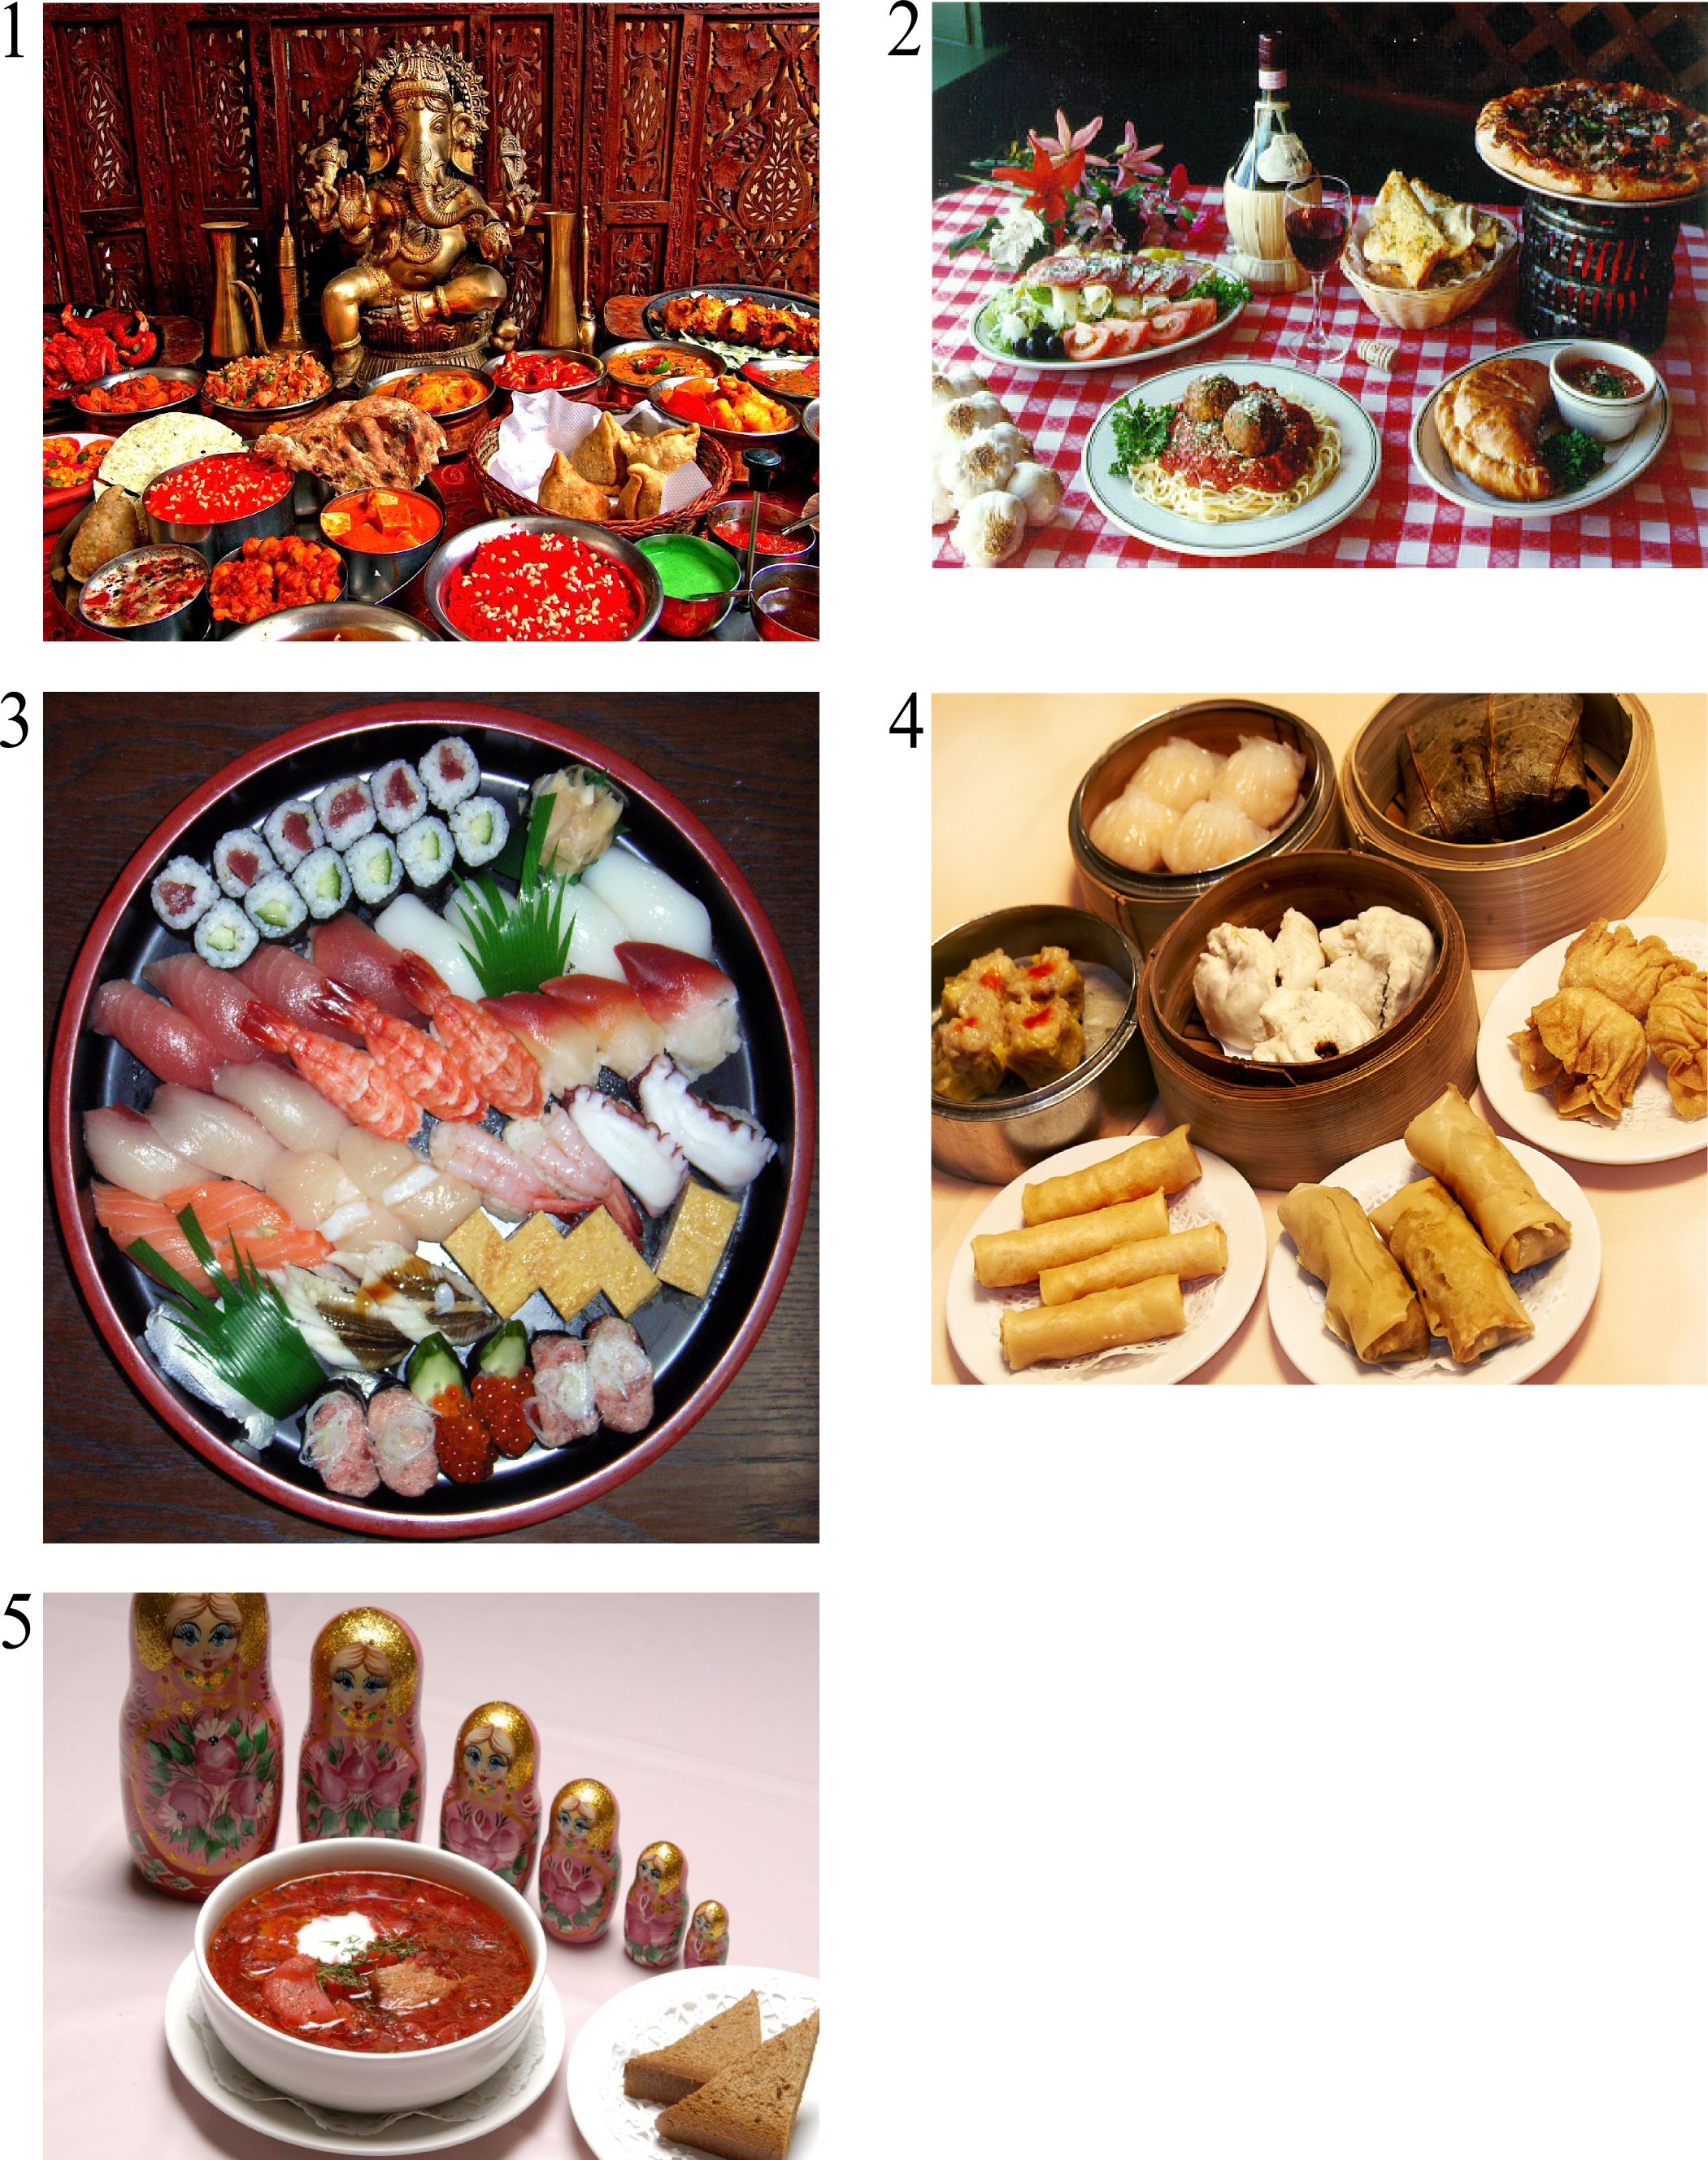
\includegraphics[scale=0.90]{figs/taskImages/testImages.jpg}
		\caption*{Figure S1: Testing image set. These images were presented 
			to all workers in the order shown after the initial set of images.}
	}
\end{figure*}

\begin{figure*}
	\centering{
	\includegraphics[scale=0.90]{figs/taskImages/ambiguous.jpg}
	\caption*{Figure S2: Ambiguous image set. These images were presented to 
		workers from certain treatments (see \textbf{Table 1}) in the main 
		text.}
	}
\end{figure*}

\begin{figure*}
	\centering{
		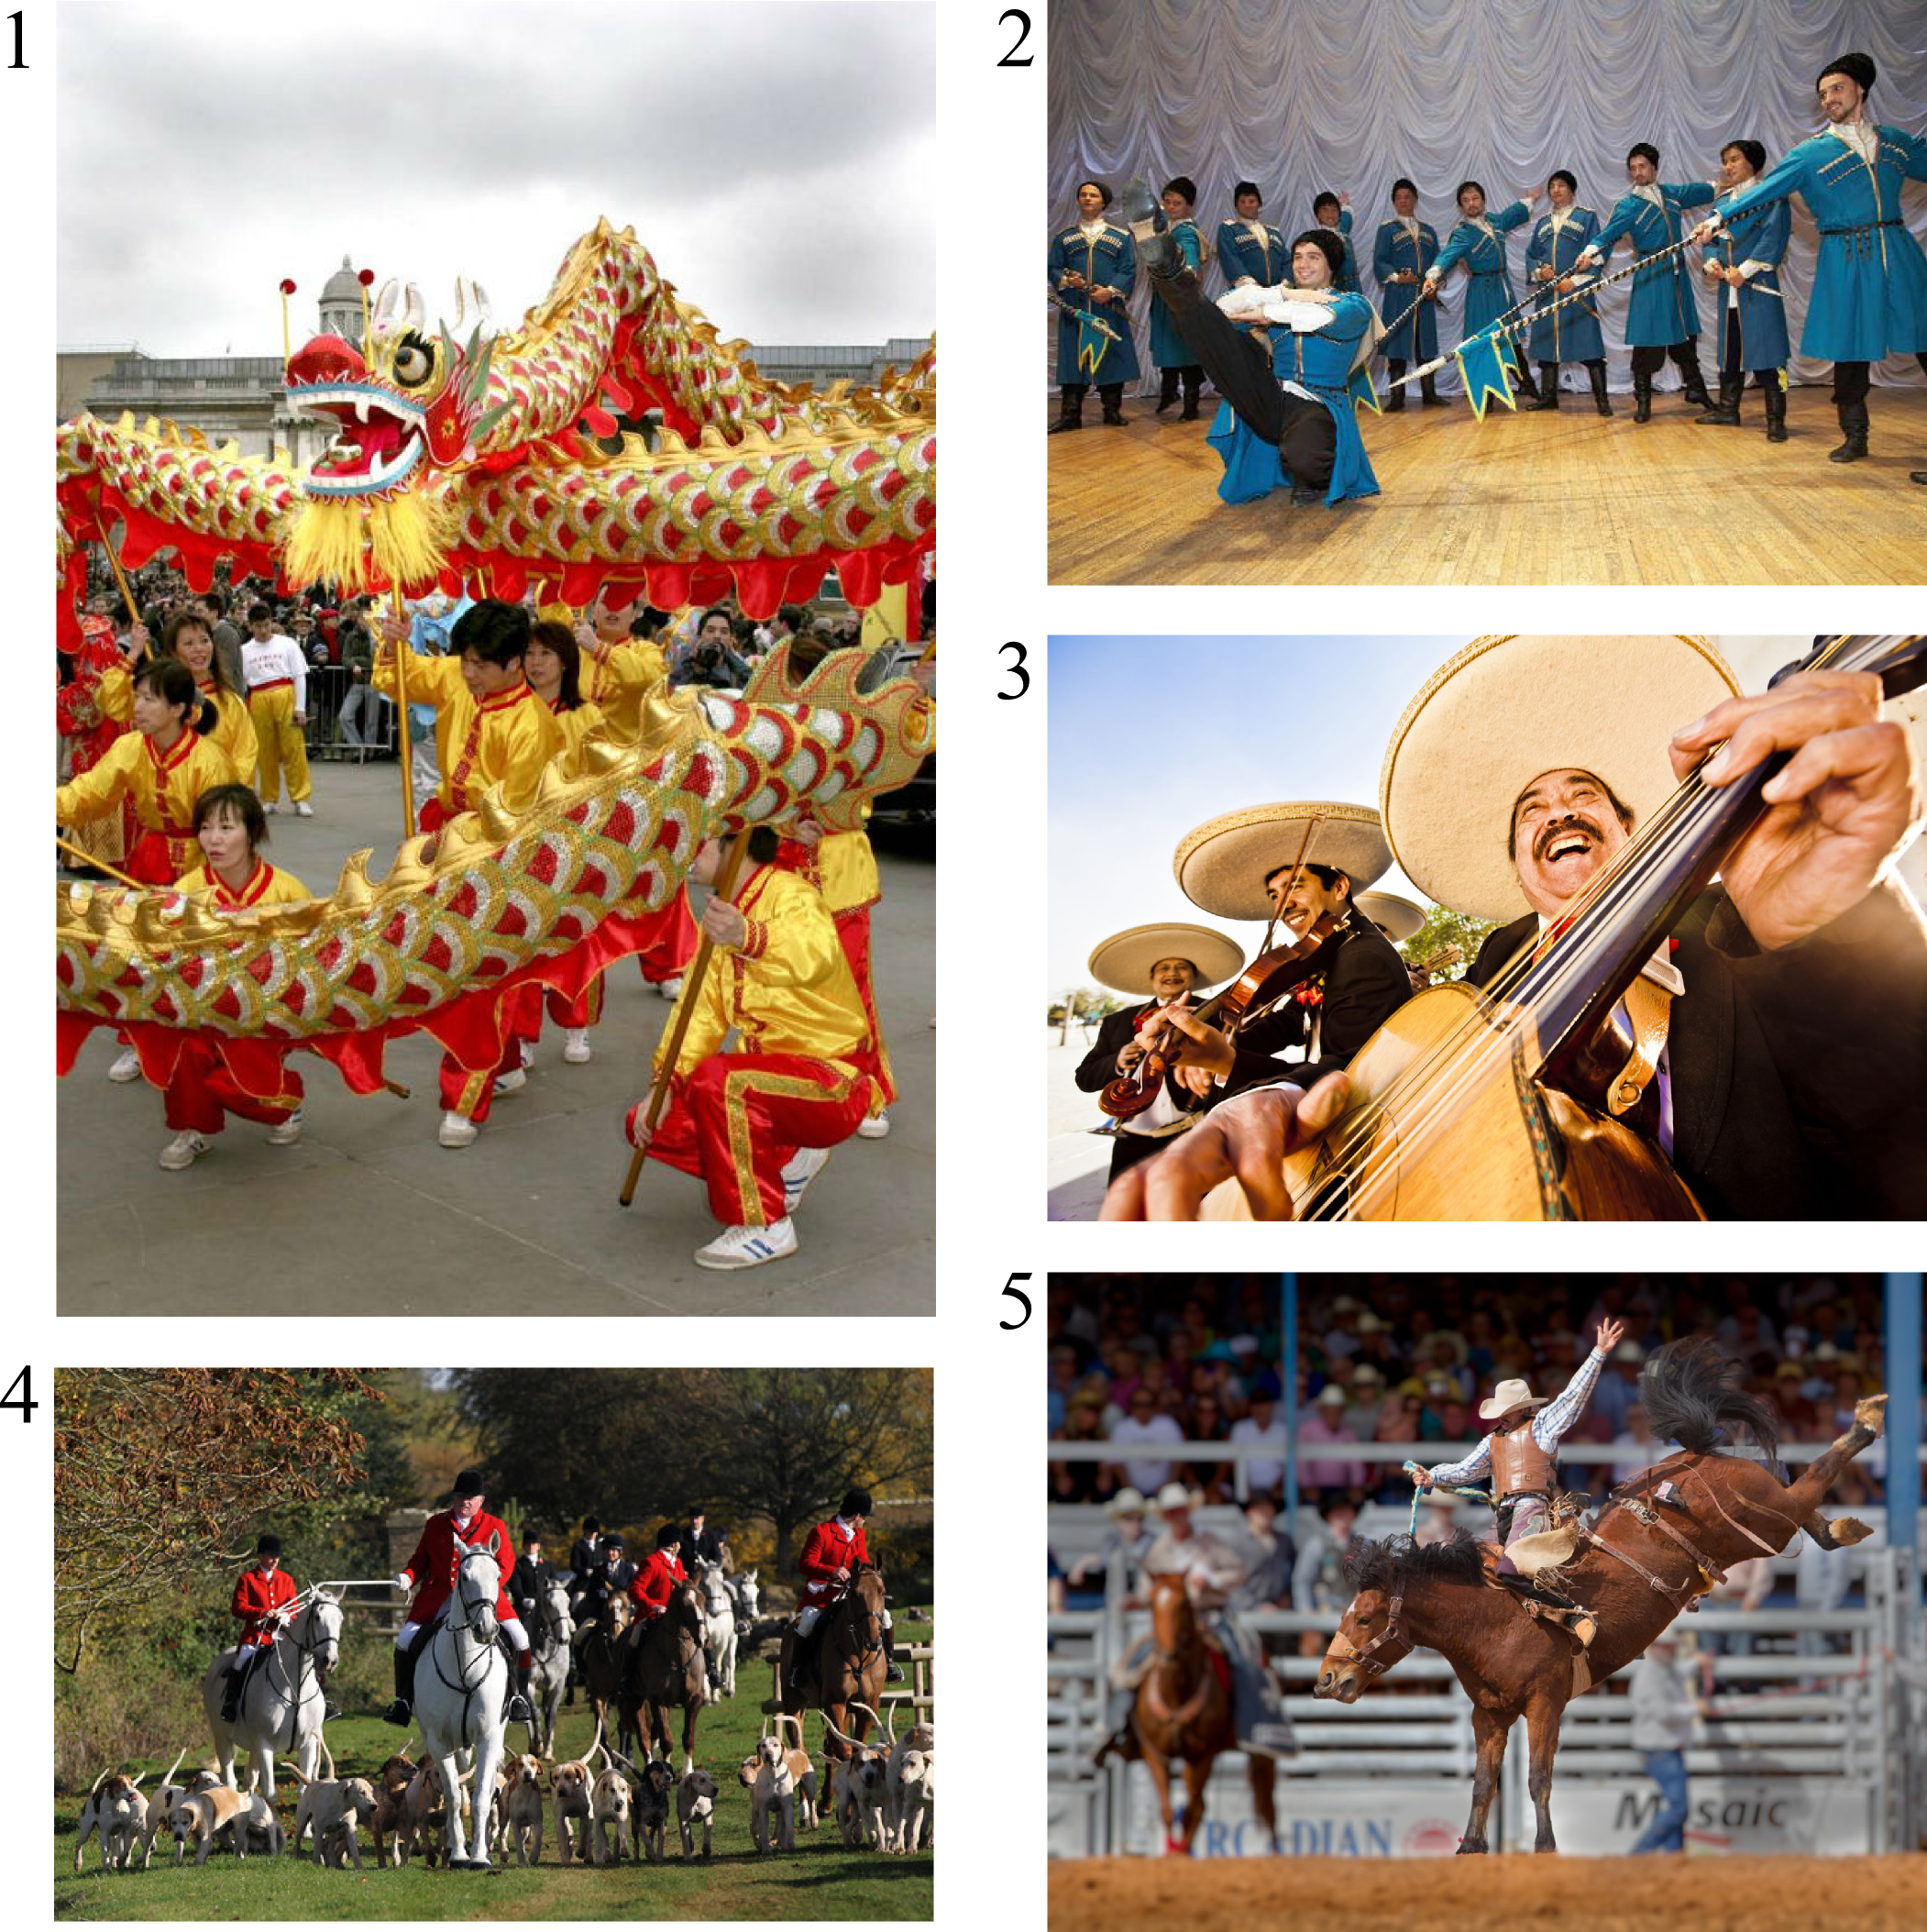
\includegraphics[scale=0.90]{figs/taskImages/cultural.jpg}
		\caption*{Figure S3: Cultural image set. These images were presented 
			to workers from certain treatments (see \textbf{Table 1}) the 
			main text.}
	}
\end{figure*}

\begin{figure*}
	\centering{
		\includegraphics[scale=0.90]{figs/taskImages/ingredients.jpg}
		\caption*{Figure S4: Ingredients image set. These images were presented
			to workers from certain treatments (see \textbf{Table 1}) in the 
			main text.}
	}
\end{figure*}
\end{document}
